The cloud-based component of this solution is designed to support multi-tenancy and multiple systems, utilizing shared cloud resources. The main principle of the multi-tenant system design is illustrated in Figure \ref{fig:multi_tenant_simple}. One tenant, for example, one factory, will be able to have multiple systems on-site, where a system refers to a group of agents, a map-service, and a broker. To optimize resource utilization, systems will also be able to share the broker, as detailed in Appendix \ref{sec:app_03}. This approach allows for efficient and effective management of the cloud resources while providing flexibility for individual tenants to have multiple systems on-site.

\begin{figure}[H]
    \centering
    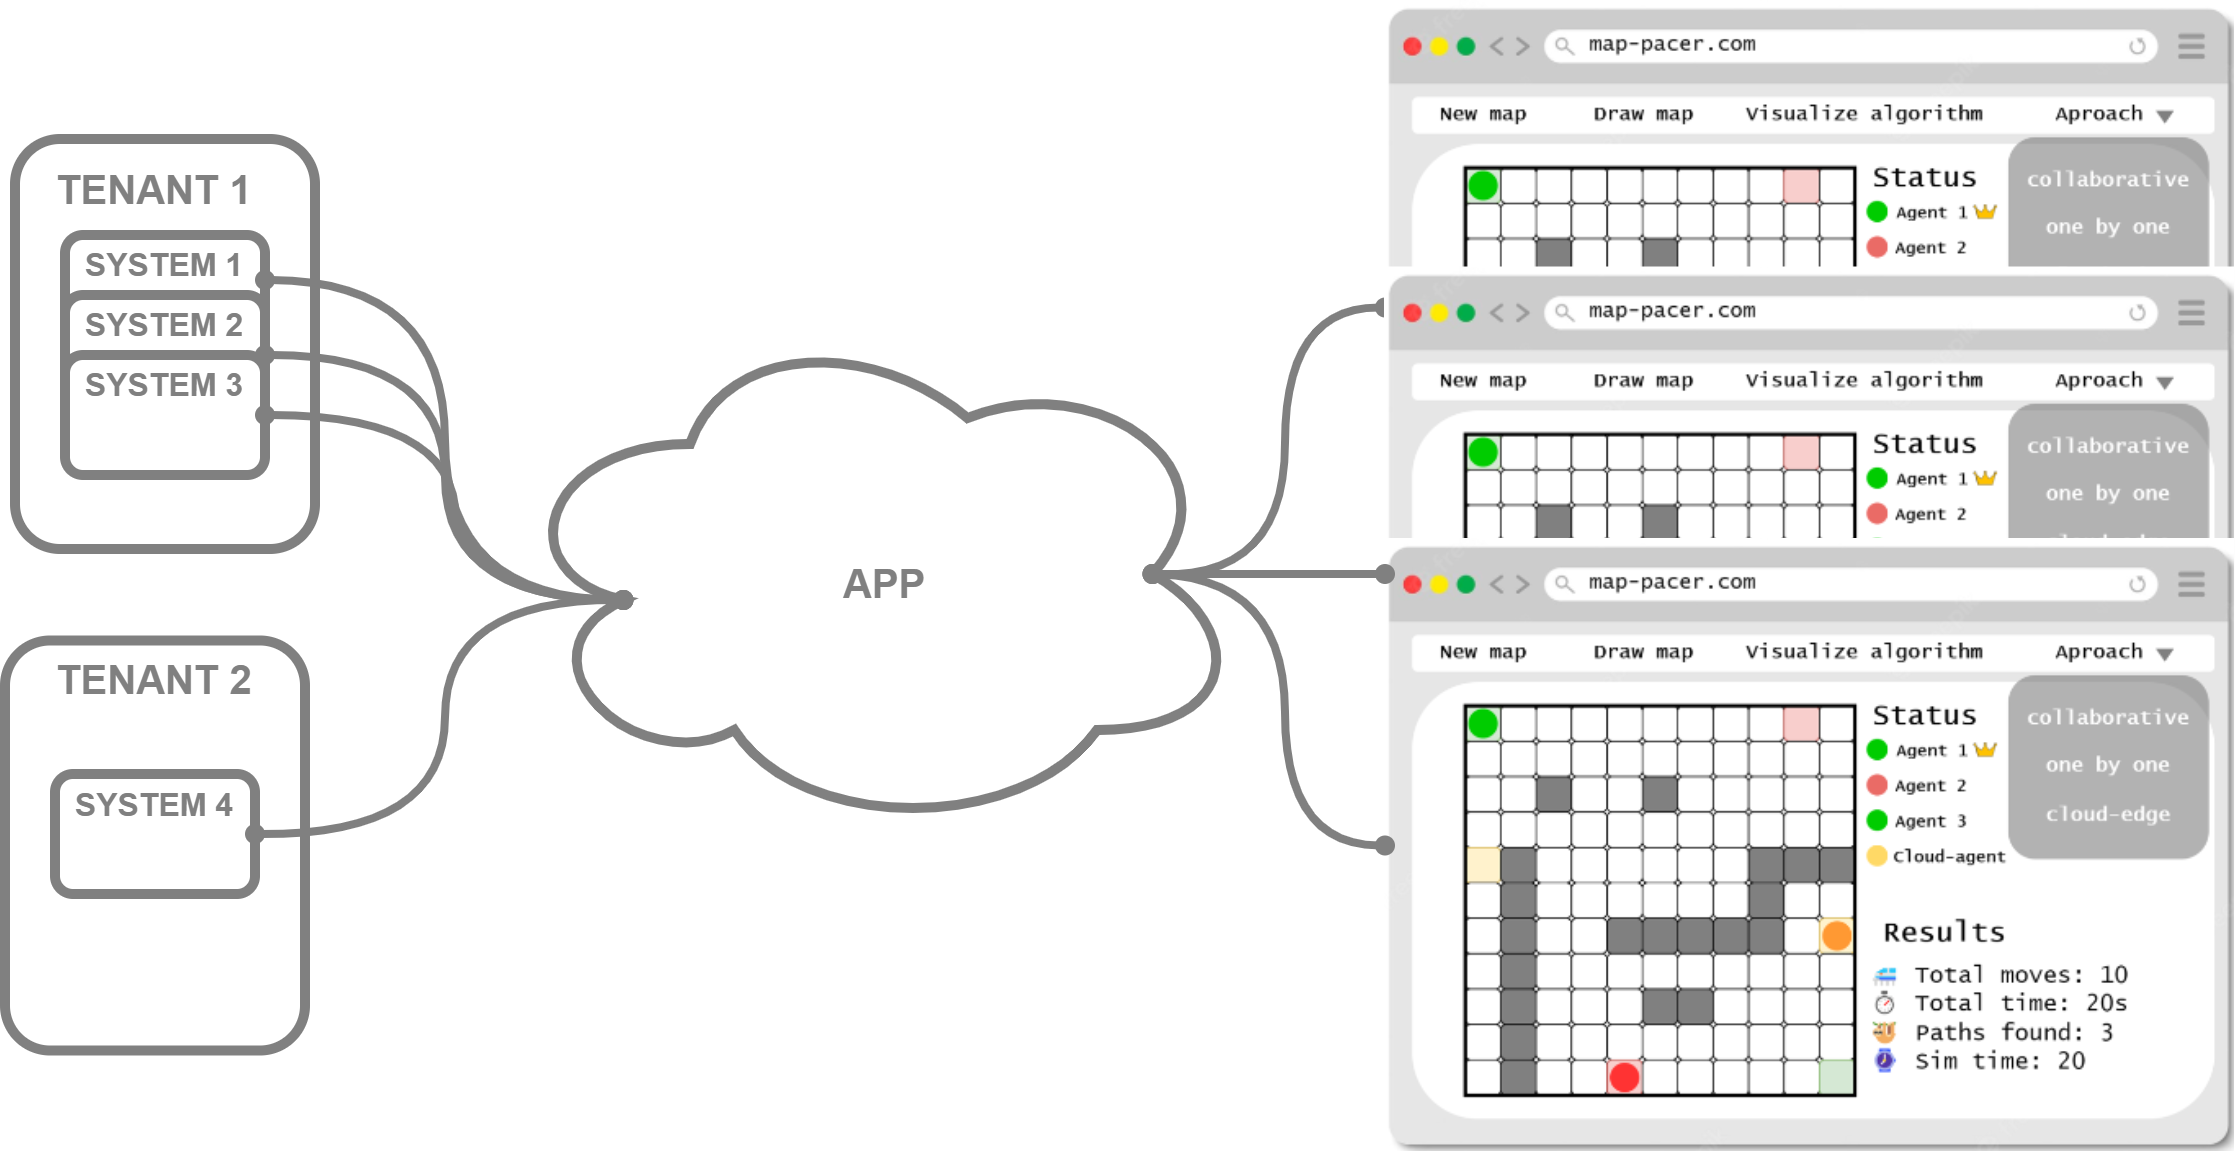
\includegraphics[width=\textwidth]{pictures/multi_tenant_simple.png}
    \caption{ Multi-tenant system design }
    \label{fig:multi_tenant_simple}
\end{figure}

The cloud components of the solution are designed to be shared among tenants and accessed through a common web-based application. The final product will include a logging page where tenants can provide credentials to authenticate themselves. Once successfully logged in, tenants will have the option to choose the system that will be visualized.

The cloud services are designed to automatically scale as more tenants are onboarded. Additionally, the microservices are implemented as stateless, with the exception of the database where all tenant data is stored. Stateless services can be easily scaled horizontally through the use of auto-scaling, providing the system with greater scalability and flexibility. This approach allows the system to accommodate an increasing number of tenants while maintaining performance and stability.